\pdfoutput=1
% ---------------------------------------------------------------------------
% Conserved amount, negotiable placement.
%
% Built for arXiv (primary class cs.SE). Everything it needs is either a
% standard LaTeX package that arXiv's TeX Live already carries, or a file in
% this directory. There is no .bib: the bibliography is a `thebibliography`
% environment at the end, so no BibTeX pass and no .bbl upload is required.
%
% Build:   pdflatex main && pdflatex main       (twice, for the references)
% Submit:  tar czf arxiv.tar.gz main.tex figures/
% ---------------------------------------------------------------------------
\documentclass[11pt,a4paper]{article}

\usepackage[T1]{fontenc}
\usepackage[utf8]{inputenc}
\usepackage{lmodern}
\usepackage[margin=2.6cm]{geometry}
\usepackage{graphicx}
\usepackage{booktabs}
\usepackage{multirow}
\usepackage{amsmath}
\usepackage{microtype}
\usepackage[hidelinks]{hyperref}
\usepackage{caption}
\captionsetup{font=small,labelfont=bf}

\newcommand{\sprg}{\textsc{Spring}}
\newcommand{\offl}{\textsc{OfficeFloor}}

\title{\bfseries Conserved amount, negotiable placement:\\
prompting moves one architecture's complexity\\
distribution and not the other's}

% Zenodo DOI, reserved before publishing and printed under the author block.
\newcommand{\thedoi}{10.5281/zenodo.22967550}
\newcommand{\doiline}{\ifdefined\thedoi\\\small\texttt{doi:\thedoi}\fi}

\author{Daniel Sagenschneider\\\small OfficeFloor\\\small\texttt{daniel@officefloor.net}\doiline}

\date{}

\begin{document}
\maketitle

\begin{abstract}
\noindent
Tesler's conservation law holds that a problem carries an irreducible amount of
complexity, and Brooks separates that essential part from the accidental part a
solution adds. If the essential part is fixed, then architecture is a question
of placement rather than quantity. This paper tests both halves of that claim
on a
controlled experiment in which an AI coding agent implements sixty accumulating
change requests against a single REST endpoint, ten independent runs per cell,
with the model held fixed. The independent variables are the architecture
(a mutative \sprg{} controller against an additive \offl{} composed pipeline)
and the instruction the agent receives, which is one of four: a bare change
request, a plain language request for cohesion, a tool that grades each change
and asks for a refactor, and the structural cost function itself pasted into
the prompt.

Across all eight cells the amount of complexity in the finished system varies
by 7\% on total Halstead volume and 15\% on total cyclomatic complexity, and
the complexity \emph{added} by the sixty rules varies by 21\% to 29\% within an
architecture. Placement does not behave this way. This paper defines a per
metric
\emph{intervention spread}, the range across the four conditions divided by
their mean, and reports the ratio of the two architectures' spreads. On amount
metrics that ratio is near 1 and no confidence interval excludes 1: both
architectures are equally immovable. On eleven placement metrics it runs from
2.9 to 10.0, and every interval lies entirely above 1, entirely because the
mutative architecture moves. Under its strongest intervention the mutative arm
arrives at the placement the additive arm occupies with no intervention at all.
The price is reported in full. Correctness fell under every intervention in both
architectures, three arrangement metrics fail to separate the arms, a
location-blind erosion measure borrowed from prior work ranks the additive
architecture worse in three of four conditions, and the placement result
predicts none of the outcome measures: the concentrated codebase was
recovered better by a cold reader in all four conditions and was cheaper to
change in three of four. The contribution is a measurable property of an
architecture, not evidence that either architecture is better.
\end{abstract}

\section{Introduction}

Larry Tesler's law of conservation of complexity holds that a problem carries
an irreducible amount of complexity, and that design moves it rather than
removing it. Tesler's own formulation, from around 1984, puts the emphasis on
placement rather than quantity: ``Every application has an inherent amount of
irreducible complexity. The only question is: who will have to deal with it,
the user, the application developer, or the platform developer?''
\cite{tesler1984, norman2010}. This paper asks Tesler's question one level
further in, of two architectures rather than of three audiences. Brooks draws
the same line from the other
direction, separating the \emph{essential} complexity that belongs to the
problem from the \emph{accidental} complexity that a particular solution adds
\cite{brooks1987}. Both claims are widely quoted and rarely measured, because
measuring them needs a setting in which the problem is genuinely held fixed
while the solution is genuinely allowed to vary.

An AI coding agent working through a fixed list of change requests is such a
setting. The task is identical by construction. The model is identical. What
can be varied is the architecture the change lands in, and the instruction the
agent is given before it writes.

This paper reports a $2 \times 4$ study. Two architectures receive sixty
accumulating change requests each, under four instruction conditions, ten
independent runs per cell: 4{,}800 agent implementations in total.

The usual question to ask of such a design is which architecture ends up with
the better structure. This paper asks a prior one. If the amount of complexity
is fixed
by the problem, then every architectural argument is an argument about
arrangement, and the interesting property of an architecture is not the
arrangement it happens to have but \emph{how far that arrangement can be moved
by anything other than the architecture itself}. An architecture whose structure
is set by the prompt, the review or the dashboard is only as durable as the
discipline applying them.

This paper contributes:

\begin{enumerate}
\item A four way measurement of Tesler conservation under a fixed task, with
  four independent operationalisations of ``amount'', reported both as finished
  totals and as the complexity the change requests added.
\item A statistic, the \emph{intervention spread}, that separates metrics
  measuring amount from metrics measuring arrangement by how far an
  intervention can move them, and a ratio between architectures that is
  approximately 1 on the former and 3 to 10 on the latter.
\item The finding that the mutative architecture's placement under its
  strongest intervention converges on the additive architecture's placement
  under no intervention.
\item A full accounting of what the interventions cost, including a correctness
  collapse in both architectures, three arrangement metrics that fail to
  separate the architectures at all, and a borrowed degradation measure that
  ranks the result the other way round.
\end{enumerate}

\section{Background and related work}

\paragraph{Complexity as a conserved quantity.} Tesler's law is normally
invoked in interface design, where the question is whether the user or the
program absorbs a step \cite{tesler1984, norman2010}. Its software engineering form is
Brooks' essence and accident distinction \cite{brooks1987}. Neither is usually
stated in a way that a measurement could falsify, which is what this study
tries to supply.

\paragraph{Measuring amount.} Four operationalisations are used, resting on
different theories, so that agreement between them is evidence rather than an
artefact of one definition: McCabe's cyclomatic complexity over control flow
\cite{mccabe1976}, Halstead volume over program vocabulary \cite{halstead1977},
weighted methods per class from the Chidamber and Kemerer suite
\cite{ck1994}, and PMD's cognitive complexity over nesting.

\paragraph{Measuring arrangement.} Concentration is measured with the
Herfindahl-Hirschman index and the Gini coefficient over per file and per class
complexity shares, which answer ``how unequally is this spread'' while staying
silent on the total. Change is measured with Hassan's change entropy
\cite{hassan2009}, applied cumulatively over the whole run rather than per
commit. Coupling is measured with CK's coupling between objects \cite{ck1994}
and with MacCormack's propagation cost \cite{maccormack2006}. The
Maintainability Index \cite{oman1992} is computed per file and averaged.
Cohesion is measured with LCOM \cite{ck1994, hs1996}.

\paragraph{Measurement under optimisation pressure.} Goodhart's law, in
Strathern's formulation, holds that a measure which becomes a target ceases to
be a good measure \cite{goodhart1975, strathern1997}. Two of the four
conditions apply deliberate optimisation pressure, and one applies it to a
disclosed formula. Which metrics survived that pressure and which did not is
therefore reported, and the optimised score itself is excluded from every
claim.

\paragraph{Agentic degradation benchmarks.} Two recent benchmarks shape this
design. The verbosity measure, and the practice of contrasting prompt arms
against a plain control, follow SlopCodeBench \cite{slopcodebench}. The strict
pass criterion, under which a checkpoint counts only when every test selected so
far is green, follows SWE-CI's gate semantics \cite{sweci}. SlopCodeBench's
whole-application erosion measure is also computed over these runs, and
Section~\ref{sec:erosion} reports it, because it points the other way. The
harness records a wider set of measures from both benchmarks, including
degradation slope, normalized change and zero regression rate; those are not
used here.

\section{The question and the statistic}

Suppose the amount of complexity is fixed by the problem. Then two
architectures that solve it differ only in arrangement, and the arrangement of
any given codebase is the joint product of the architecture and everything else
that shaped it: the prompt, the review, the metric on the dashboard. An
architecture whose arrangement is substantially determined by those other
things is one whose structure is only as durable as the discipline applying
them. An architecture whose arrangement is determined by its own composition is
not.

That is an empirical question, and it needs a statistic. For a metric $m$ and
an architecture $a$, let $\mu_{c}(m,a)$ be the mean over ten runs of the
per run mean of $m$ over the final phase, under condition $c$. The
\textbf{intervention spread} is

\begin{equation}
S(m,a) \;=\; \frac{\max_{c} \mu_{c}(m,a) \;-\; \min_{c} \mu_{c}(m,a)}
                  {\left|\overline{\mu_{c}(m,a)}\right|}
\end{equation}

where $c$ ranges over the four conditions, and the \textbf{plasticity ratio}

\begin{equation}
R(m) \;=\; S(m,\ \sprg{})\ /\ S(m,\ \offl{}).
\end{equation}

$S$ asks how far an intervention moved an architecture on that metric,
expressed relative to the metric's own level so that metrics on different
scales are comparable. $R$ asks whether the two architectures were moved
equally. Under Tesler conservation, amount metrics should have small $S$ for
both architectures, and therefore $R \approx 1$. The thesis of this paper is
that placement metrics have $R \gg 1$.

Both are computed over four condition means, each itself a mean over ten runs,
so both carry sampling error. An interval is attached by a \textbf{cluster
bootstrap over chains}: within each of the eight cells the ten chains are
resampled with replacement, the cell mean recomputed, and $S$ and $R$ recomputed
from the resampled means, 10{,}000 times. The reported interval is the 2.5th to
97.5th percentile of that distribution.

The chain is the resampling unit, not the checkpoint. Checkpoints within a chain
are successive states of one codebase and are strongly dependent, so treating
them as independent would give intervals far too narrow. Chains are independent
runs. Each cell is resampled separately, because chain $k$ of one condition has
no relationship to chain $k$ of another.

\section{Study design}

\paragraph{Task.} A fixed plan of sixty change requests, each adding or
revising a business rule on one endpoint, \texttt{POST /api/owners}, of the
Spring PetClinic REST application. The plan and its acceptance suite were
frozen on 2026-08-08, before the earliest of the four runs reported here, so
all four conditions faced an identical task.

\paragraph{Architectures.} The \emph{mutative} arm is an idiomatic Spring
\cite{spring} \texttt{@RestController}: a rule is a statement added to a
handler method. The \emph{additive} arm is the same application built with
OfficeFloor \cite{officefloor}, a framework whose endpoints are YAML composed
graphs of functions, so a rule is a new function and a new edge. Both arms implement the same sixty rules and are held to the same
black box acceptance suite, which the agent never sees.

\paragraph{Agent.} \texttt{claude-opus-4-8}, held fixed across all cells. Each
change request is a fresh session with no memory of the previous one, so the
agent re-reads whatever it needs from the code itself. Nothing but the code
crosses between checkpoints.

\paragraph{Conditions.} Four, each a full sweep of both architectures at ten
runs each, each changing exactly one lever:

\begin{enumerate}
\item \texttt{just-solve}. Control. The change request and nothing else.
\item \texttt{cohesion-prompt}. The \emph{prompt} lever. One plain language
  paragraph asking for well structured code. No metric is named and the
  experiment is not mentioned.
\item \texttt{impact-gated}. The \emph{tool} lever. A neutral implement prompt,
  but a change that grades badly gets one quality gated refactor guided by the
  flagged locations, then is accepted whatever its grade. The gate fired on 195
  of 1{,}200 checkpoints.
\item \texttt{formula-provided}. The \emph{disclosure} lever. The structural
  cost function itself pasted into the implement prompt as the objective. Its
  gate fired on 3 of 1{,}200 checkpoints, so this condition is the prompt
  lever, measured.
\end{enumerate}

\paragraph{Measurement.} Every metric is recomputed from the committed source
at every checkpoint by \texttt{lizard}, PMD, CK \cite{ck-tool} and
\texttt{jscpd}, never read back from anything the agent wrote. The population
is production Java only. OfficeFloor's YAML wiring is counted in a separate
pool and is never folded into a Java denominator, because doing so would let a
wiring based architecture dilute any per line metric.

\paragraph{Aggregation.} A run is binned into fifths of twelve change requests.
Unless stated otherwise, every reported value is the final phase, meaning
change requests 49 to 60, averaged within a run first and then across the ten
runs, so that a run missing a checkpoint does not get a smaller vote than a
complete one. Parenthesised figures are one standard deviation across the ten
runs.

\paragraph{Scale.} 4 conditions $\times$ 2 architectures $\times$ 10 runs
$\times$ 60 change requests = 4{,}800 agent implementations, at a total
implement turn model spend of \$6{,}815.

\section{Results}

\subsection{The amount is conserved}

Table~\ref{tab:amount} gives the four amount operationalisations for all eight
cells. They rest on different theories and different tools, and they agree.
Total Halstead volume varies by 7\% across all eight cells, total cyclomatic
complexity by 15\%. No condition reached under the floor, in either
architecture.

\begin{table}[t]
\centering
\caption{Amount of complexity in the finished system, final phase, mean (SD)
over ten runs. ``Spread'' is the range over all eight cells divided by their
mean.}
\label{tab:amount}
\scriptsize
\setlength{\tabcolsep}{4pt}
\begin{tabular}{llrrrrr}
\toprule
Metric & Arch & \texttt{just-solve} & \texttt{cohesion} & \texttt{gated} & \texttt{formula} & Spread \\
\midrule
\texttt{total\_cc} & \sprg{}  & 652 (21) & 694 (17) & 646 (23) & 642 (38) & \multirow{2}{*}{15\%} \\
                   & \offl{}  & 656 (12) & 681 (28) & 641 (20) & 597 (19) & \\
\addlinespace
\texttt{halstead\_volume} & \sprg{} & 215{,}300 (6{,}410) & 220{,}800 (6{,}480) & 209{,}000 (5{,}410) & 206{,}100 (12{,}300) & \multirow{2}{*}{7\%} \\
                          & \offl{} & 216{,}600 (1{,}310) & 221{,}500 (2{,}110) & 214{,}100 (3{,}910) & 207{,}800 (1{,}690) & \\
\addlinespace
\texttt{ck\_wmc\_total} & \sprg{} & 762 (20) & 826 (18) & 761 (21) & 750 (38) & \multirow{2}{*}{20\%} \\
                        & \offl{} & 738 (12) & 766 (27) & 725 (21) & 679 (17) & \\
\addlinespace
\texttt{pmd\_cognitive\_total} & \sprg{} & 323 (14) & 293 (12) & 293 (11) & 283 (24) & \multirow{2}{*}{18\%} \\
                               & \offl{} & 319 (17) & 289 (22) & 310 (23) & 268 (14) & \\
\bottomrule
\end{tabular}
\end{table}

Finished totals are the quantity a team maintains, but the two applications do
not start level. Each arm begins from one fixed commit, identical for all four
conditions, and at that commit the mutative arm carries 404 points of cyclomatic
complexity across 55 files and the additive arm 351 across 120. A matching
total is therefore not automatically a matching amount of work, and
Table~\ref{tab:added} repeats the test on the complexity the sixty rules
\emph{added}.

\begin{table}[t]
\centering
\caption{Complexity added by the sixty change requests, computed per run as the
final phase mean minus the value at that arm's \texttt{base\_ref}, the commit
every run starts from. That base is one fixed codebase per arm, identical across
all four conditions, so the SD shown is the between run spread at the end. Mean
(SD) over ten runs. ``Spread'' is within an architecture, across the four
conditions.}
\label{tab:added}
\scriptsize
\setlength{\tabcolsep}{4pt}
\begin{tabular}{llrrrrr}
\toprule
Metric & Arch & \texttt{just-solve} & \texttt{cohesion} & \texttt{gated} & \texttt{formula} & Spread \\
\midrule
\texttt{total\_cc} & \sprg{} & 248 (21) & 290 (17) & 242 (23) & 238 (38) & 21\% \\
                   & \offl{} & 305 (12) & 330 (28) & 290 (20) & 246 (19) & 29\% \\
\addlinespace
\texttt{halstead\_volume} & \sprg{} & 59{,}021 (6{,}406) & 64{,}544 (6{,}480) & 52{,}700 (5{,}406) & 49{,}847 (12{,}324) & 26\% \\
                          & \offl{} & 61{,}287 (1{,}305) & 66{,}174 (2{,}107) & 58{,}803 (3{,}915) & 52{,}507 (1{,}691) & 23\% \\
\addlinespace
\texttt{ck\_wmc\_total} & \sprg{} & 244 (20) & 308 (18) & 243 (21) & 232 (38) & 29\% \\
                        & \offl{} & 307 (12) & 334 (27) & 294 (21) & 248 (17) & 29\% \\
\bottomrule
\end{tabular}
\end{table}

The conservation claim survives the stricter test and picks up a qualifier. The
spread widens from 7\% on totals to between 21\% and 29\% on what was added, so
the honest statement is that the amount is \emph{steady} rather than fixed. And
the additive architecture added more complexity than the mutative one in every
condition. That is the price of a composed pipeline. It is a real cost, and it
is visible before any argument about placement begins. The additive arm's
advantage is not that it carries less. It is that its baseline was lower and it
stayed where it was put.

\subsection{The placement is not}

Table~\ref{tab:spread} gives the intervention spread for both architectures and
the plasticity ratio between them, for eleven placement metrics and, for
contrast, the amount metrics from Table~\ref{tab:amount}.
Figure~\ref{fig:plasticity} shows the same result.

\begin{table}[t]
\centering
\caption{Intervention spread $S$ per architecture, and the plasticity ratio
$R$. Final phase. A ratio near 1 means the four conditions moved both
architectures equally.}
\label{tab:spread}
\small
\begin{tabular}{lrrrr}
\toprule
Metric & $S(\sprg{})$ & $S(\offl{})$ & $R$ & 95\% CI for $R$ \\
\midrule
\multicolumn{5}{l}{\emph{Placement}}\\
\texttt{cum\_change\_top1}         & 110\% & 11\% & 10.0 & [4.13, 30.35] \\
\texttt{cum\_change\_entropy\_norm} & 24\% &  3\% &  9.2 & [6.21, 14.67] \\
\texttt{cum\_change\_hhi}          & 142\% & 20\% &  7.3 & [4.17, 11.32] \\
\texttt{ccdist\_file\_top1}        &  87\% & 17\% &  5.3 & [2.57, 9.23] \\
\texttt{ck\_cbo\_mean}             &  14\% &  3\% &  4.2 & [2.59, 6.48] \\
\texttt{ccdist\_file\_gini}        &  34\% &  8\% &  4.1 & [3.24, 5.43] \\
\texttt{total\_files}              &  37\% &  9\% &  4.0 & [2.87, 5.50] \\
\texttt{ccdist\_file\_hhi}         & 106\% & 28\% &  3.7 & [2.70, 5.45] \\
\texttt{node\_cc\_median}          &  87\% & 24\% &  3.5 & [2.03, 6.16] \\
\texttt{wmcdist\_class\_hhi}       & 100\% & 29\% &  3.4 & [2.53, 4.98] \\
\texttt{propagation\_cost}         &  36\% & 12\% &  2.9 & [1.06, 9.27] \\
\midrule
\multicolumn{5}{l}{\emph{Amount}}\\
\texttt{halstead\_volume}          &   7\% &  6\% &  1.1 & [0.67, 1.70] \\
\texttt{java\_loc}                 &  11\% & 10\% &  1.1 & [0.73, 1.42] \\
\texttt{total\_fns}                &  15\% & 16\% &  1.0 & [0.75, 1.22] \\
\texttt{pmd\_cognitive\_total}     &  13\% & 17\% &  0.8 & [0.49, 1.18] \\
\texttt{ck\_wmc\_total}            &  10\% & 12\% &  0.8 & [0.60, 1.18] \\
\texttt{total\_cc}                 &   8\% & 13\% &  0.6 & [0.43, 0.98] \\
\midrule
\multicolumn{5}{l}{\emph{Arrangement metrics that do not separate the architectures}}\\
\texttt{ck\_lcom\_mean}            &  65\% & 47\% &  1.4 & -- \\
\texttt{ccdist\_fn\_gini}          &  15\% & 14\% &  1.1 & -- \\
\texttt{cogdist\_fn\_gini}         &  16\% & 16\% &  1.0 & -- \\
\bottomrule
\end{tabular}
\end{table}

\begin{figure}[t]
\centering
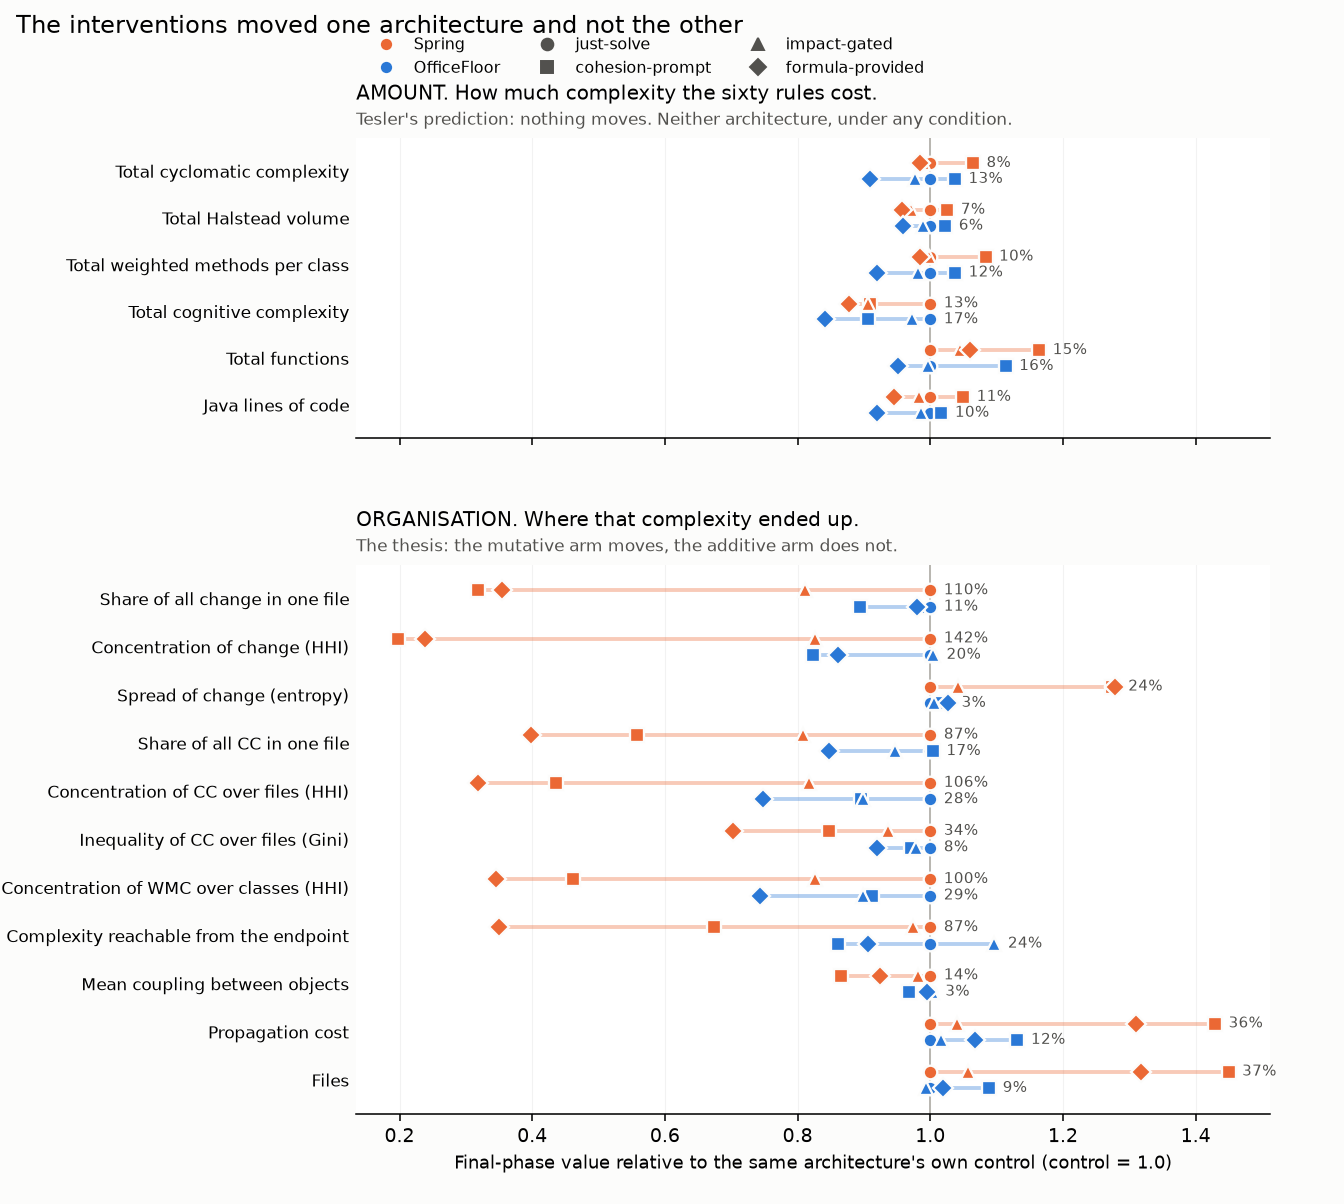
\includegraphics[width=\textwidth]{figures/plasticity.png}
\caption{Every condition's final phase value divided by the same
architecture's own control, so 1.0 means the intervention changed nothing. Top
panel is amount, where neither architecture moves. Bottom panel is placement,
where one does. Normalising to each architecture's own control is deliberate,
because the question is how far each moved rather than where it started;
absolute levels are in Tables~\ref{tab:amount} and \ref{tab:convergence}.}
\label{fig:plasticity}
\end{figure}

The separation is clean, and it survives the interval. On the eleven placement
metrics $R$ lies between 2.9 and 10.0, and \textbf{all eleven have a 95\%
confidence interval lying entirely above 1}. On the six amount metrics $R$ lies
between 0.6 and 1.1 and \textbf{not one interval excludes 1}, which is the
conservation result restated as a test rather than as an observation. The amount
group is an internal control that behaves as it should: it was predicted to show
no asymmetry, and it shows none.

Two of the eleven deserve less weight than the rest.
\texttt{propagation\_cost} only just clears the line at [1.06, 9.27], and
\texttt{cum\_change\_top1}'s interval spans [4.13, 30.35], which is the small
denominator instability discussed in Section~\ref{sec:threats} made visible.
The conclusion rests on neither: nine of the eleven have a lower bound above
2.

The third group is reported because it does not fit. Two distribution measures
taken over individual functions rather than over files or classes,
\texttt{ccdist\_fn\_gini} and \texttt{cogdist\_fn\_gini}, move by the same
amount in both architectures, which suggests the inequality of complexity
\emph{within} a population of functions is architecture neutral and that the
signal lives at the level where the architectural decision is actually made.
\texttt{ck\_lcom\_mean} is the more awkward one: cohesion is what the
plain-language prompt asked for by name, and it separates the arms less than
almost anything else in the table. It also improved most under the condition
that never mentioned it, falling from 29.6 to 17.3 in the mutative arm under the
formula against 26.0 under the cohesion prompt.

\subsection{The whole distribution, not the chosen eleven}

Eleven metrics out of a much larger set were chosen by the author, so the
obvious question is what the rest do. Figure~\ref{fig:dist} answers it for
every metric the study records.

\begin{figure}[t]
\centering
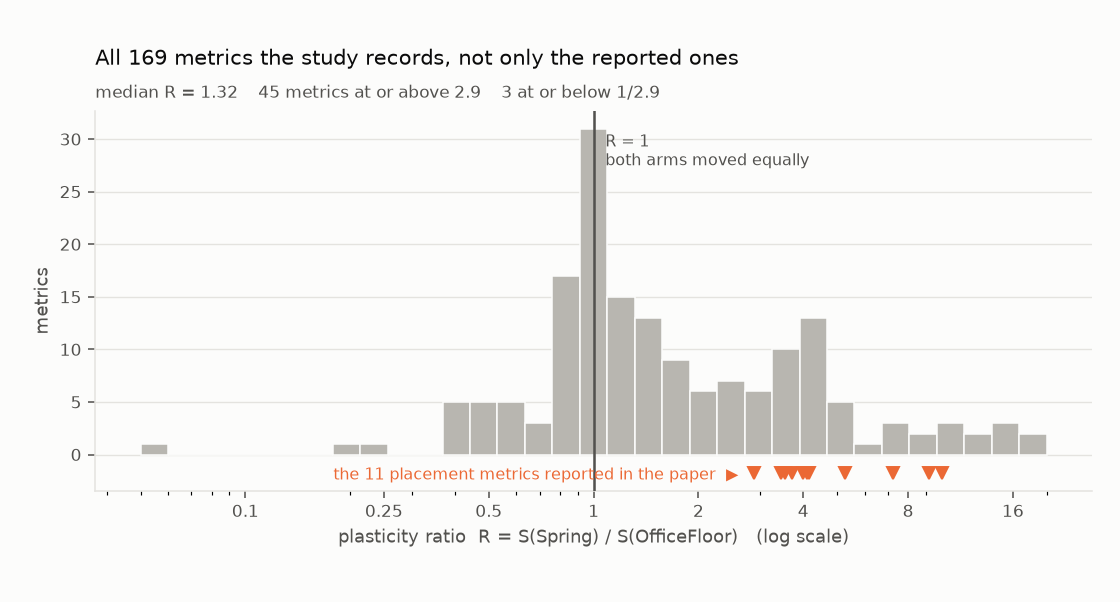
\includegraphics[width=\textwidth]{figures/plasticity_dist.png}
\caption{The plasticity ratio for all 169 metrics with a computable $R$, on a
log scale so that halving and doubling are the same distance from parity. The
markers show where the eleven reported placement metrics fall.}
\label{fig:dist}
\end{figure}

Two things follow, and they point in opposite directions. The direction of the
effect is robust: 116 of 169 metrics have $R \ge 1$, only 3 fall at or below
$1/2.9$, and 45 reach or exceed 2.9, which is the weakest ratio the paper
reports. There is no selection of eleven metrics from this set that would
reverse the sign of the result.

The magnitude is not robust in the same way. The median metric gives
$R = 1.32$, and the reported eleven sit in the upper tail rather than at the
centre. The honest reading is that the asymmetry is pervasive and usually mild,
and that it is large on the specific family of metrics that measure
concentration of complexity and of change. That is the claim the paper makes,
but a reader should take the 2.9 to 10.0 range as describing that family and
not as describing measurement of this codebase in general.

\subsection{A location-blind metric points the other way}
\label{sec:erosion}

One measure from the benchmarks this design borrows from contradicts the result,
and it is reported here rather than left out. SlopCodeBench's whole-application
\emph{erosion} is the share of total complexity mass held by functions above a
cyclomatic threshold. Measured over the same runs it ranks the additive arm as
the more eroded one in three of the four conditions.

\begin{center}
\small
\begin{tabular}{lrrl}
\toprule
Condition & \sprg{} & \offl{} & scored worse \\
\midrule
\texttt{just-solve}       & 0.087 & 0.126 & \offl{} \\
\texttt{cohesion-prompt}  & 0.048 & 0.043 & \sprg{} \\
\texttt{impact-gated}     & 0.044 & 0.058 & \offl{} \\
\texttt{formula-provided} & 0.008 & 0.023 & \offl{} \\
\bottomrule
\end{tabular}
\end{center}

\noindent This is not an anomaly that the argument has to survive. It is what
the argument predicts. Erosion is location-blind by construction: it cannot
distinguish a cyclomatic complexity of 19 sitting in a god method from the same
19 sitting in an isolated single-responsibility algorithm. The whole claim of
this paper is that measures of that kind cannot see placement, and erosion is
one of them.

The mechanism is visible in the change request plan. Eight of the sixty rules
concern E.164 phone normalisation, three concern Luhn checksums and two concern
soundex matching. These are self-contained algorithms with genuinely high branch
counts, both arms must implement them, and neither architecture makes them
simpler. They therefore dominate the numerator. The count of functions over the
threshold moves the same way, 3.3 in the additive arm against 1.7 in the
mutative one under the control, which is what spreading the same work across
more units does to a threshold count.

So a reader who prefers erosion to the placement family would reach the opposite
conclusion from this data. We think that preference is mistaken, for the reason
above, and Section~\ref{sec:threats} states the case a reader would have to
accept to hold it. The metric is recorded by the harness for every checkpoint of
every run and is in the published data.

\subsection{The mutative arm converges on the additive arm's untouched position}

The interventions worked. Table~\ref{tab:convergence} shows what ``worked''
converged on. The comparison throughout is against the additive arm under the
control condition, not against either arm's starting commit.

\begin{table}[t]
\centering
\caption{Final phase placement. ``Best'' is whichever of the three
interventions scored best on that metric for the mutative arm, and ``from''
names it. ``\offl{} control'' is the additive arm with no intervention at all.
The last column says which of those two is still ahead.}
\label{tab:convergence}
\footnotesize
\setlength{\tabcolsep}{4pt}
\begin{tabular}{lrrlrl}
\toprule
Metric & \sprg{} ctl & \sprg{} best & from & \offl{} \emph{ctl} & ahead \\
\midrule
\texttt{cum\_change\_top1}          & 0.344 & 0.110 & cohesion & 0.106 & \offl{} \\
\texttt{ccdist\_file\_top1}         & 0.197 & 0.078 & formula  & 0.086 & \sprg{} \\
\texttt{ccdist\_file\_hhi}          & 0.0727 & 0.0232 & formula & 0.0217 & \offl{} \\
\texttt{wmcdist\_class\_hhi}        & 0.0554 & 0.0191 & formula & 0.0182 & \offl{} \\
\texttt{cum\_change\_entropy\_norm} & 0.721 & 0.921 & formula & 0.886 & \sprg{} \\
\bottomrule
\end{tabular}
\end{table}

Coaching brings the mutative architecture to roughly the placement the additive
architecture occupies with none. ``Roughly'' is the right word and the table is
shown at full precision so it can be checked: on three of the five metrics the
additive arm's untouched control is still ahead of the mutative arm's best, and
on two the mutative arm passes it. The claim is convergence on the same
neighbourhood, not that coaching closes the gap exactly.

Two caveats attach to this table and neither is small. The best of three is a
maximum over conditions, which is biased upward when each cell carries run to
run noise, and no correction is applied. And the winning condition differs by
row, four from the formula and one from the cohesion prompt, so no single
intervention achieves the whole of this. Read the table as showing what the
best available coaching reaches, metric by metric, rather than as the profile of
any one condition.

\subsection{What the interventions cost}

\paragraph{Correctness.} The strict pass rate, meaning every test of every rule
so far is green, fell under every intervention in both architectures. The
mutative arm went from 0.267 under the control to 0.108 under the cohesion
prompt and 0.033 under the formula; the additive arm went from 0.325 to 0.050
under the cohesion prompt. Both architectures are plastic here
($R = 1.1$), and structural stability did not buy safety.

These particular means need more care than the rest of the paper, because the
underlying distribution is bimodal and the mean falls in a gap where almost no
run lands. In every one of the eight cells most runs finish at 0 or 0.167 and
two or three finish near 0.9. The mutative control mean of 0.267 is three runs
at 0, five at 0.167 and two at 0.917, as Figure~\ref{fig:strictpass} shows.
The ordering between conditions survives,
because the count of runs stuck at 0 moves the same way the mean does, from 3
of 10 under the control to 8 of 10 under the formula. The level does not.

\begin{figure}[t]
\centering
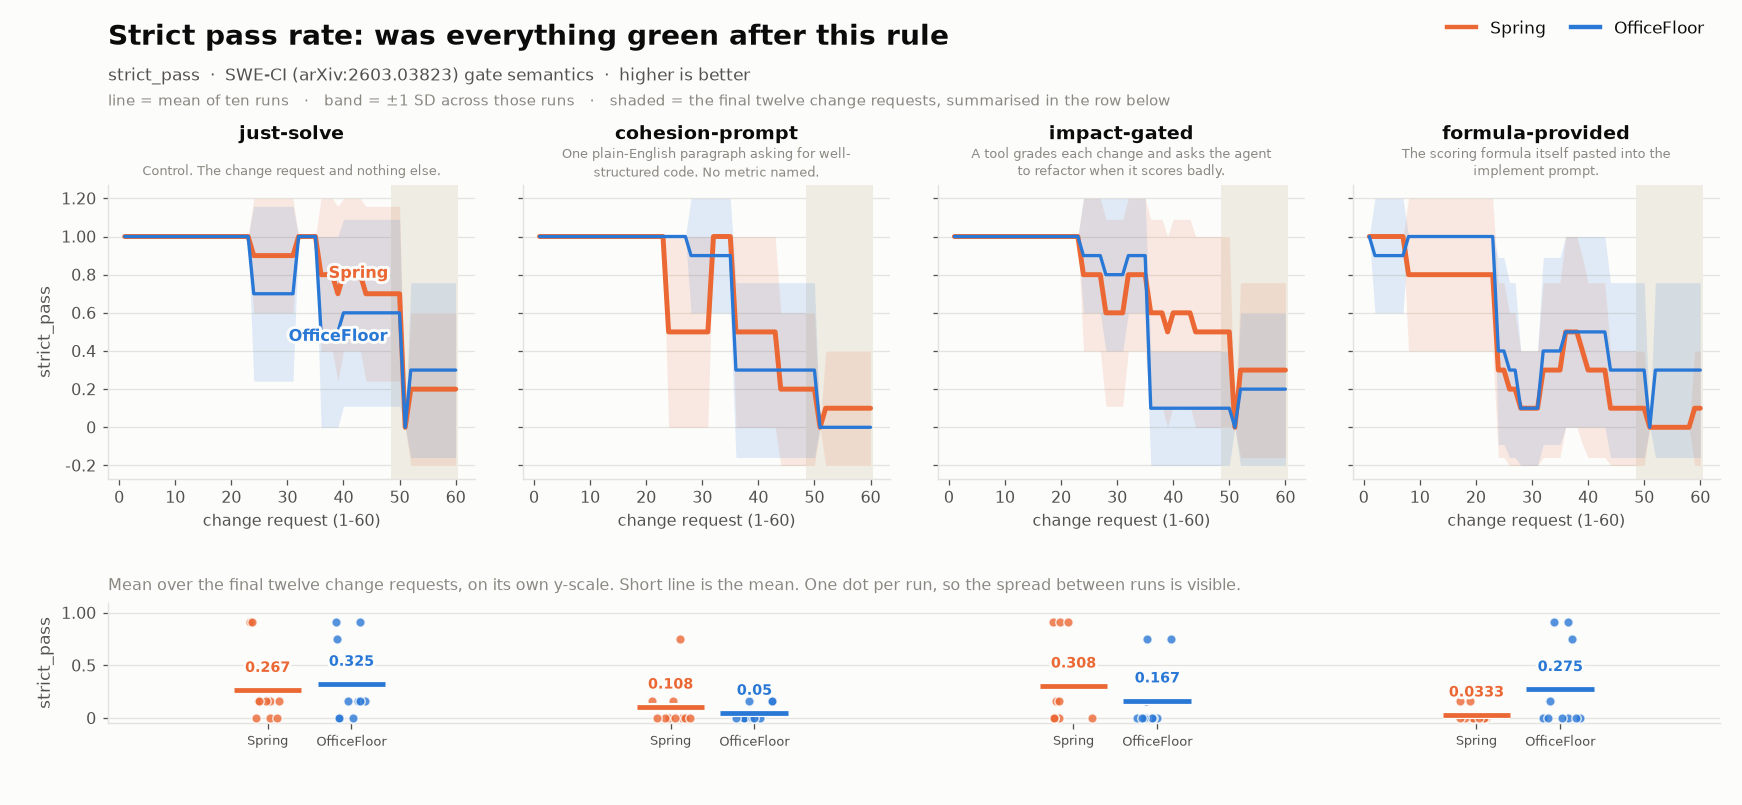
\includegraphics[width=\textwidth]{figures/strict_pass.png}
\caption{Strict pass rate. The four panels are the trajectory over the sixty
change requests. The row beneath puts the eight final phase means side by side
with one dot per run, which is where the bimodality is visible: in every cell
most runs sit at 0 or 0.167 while two or three sit near 0.9, so the mean falls
in a gap where almost no run lands.}
\label{fig:strictpass}
\end{figure}

\paragraph{Escape from the call graph.} Under the formula condition the
mutative arm's count of container dispatched classes, meaning advice, aspects,
filters and entity listeners, rose from 3.0 (SD 0) to 11.2 (SD 9.4) per run.
That is complexity leaving the call graph rather than leaving the codebase, and
it is why no single call graph scoped metric is treated as decisive here. The
additive arm's count is exactly 1.0 in all four conditions.

\paragraph{Duplication.} Verbosity rose in the mutative arm from 0.851 to 1.002
under the cohesion prompt and 0.991 under the formula, on a codebase that did
not grow. Distributing logic across more units creates the opportunity to copy
between them, and it was taken.

\paragraph{Money.} Cost per run rose under the cohesion prompt, from \$78.40 to
\$96.73 in the mutative arm and \$86.51 to \$101.18 in the additive arm, and
fell slightly under the formula.

\subsection{What the placement result does not predict}
\label{sec:nopredict}

The reason to care about placement is the belief that it governs what a team
experiences: comprehension, cost, time, safety. On this study's own outcome
measures that belief is not supported, and the direction is against the
additive architecture rather than merely absent.

\begin{table}[t]
\centering
\caption{Outcome measures, final phase, mean (SD) over ten runs. These are
levels, not spreads. \texttt{probe\_recall} is a read only comprehension probe:
a fresh agent, given the finished codebase and none of the history, is asked to
recover the rules, and higher is better. The other two are lower is better.}
\label{tab:outcome}
\scriptsize
\setlength{\tabcolsep}{4pt}
\begin{tabular}{llrrrrc}
\toprule
Metric & Arch & \texttt{just-solve} & \texttt{cohesion} & \texttt{gated} & \texttt{formula} & \sprg{} better in \\
\midrule
\texttt{probe\_recall} & \sprg{} & 0.639 (0.111) & 0.573 (0.040) & 0.590 (0.055) & 0.688 (0.055) & \multirow{2}{*}{\textbf{4 of 4}} \\
                       & \offl{} & 0.602 (0.025) & 0.555 (0.060) & 0.589 (0.071) & 0.613 (0.045) & \\
\addlinespace
\texttt{cost\_usd} & \sprg{} & 1.64 (0.10) & 2.01 (0.18) & 1.68 (0.19) & 1.51 (0.13) & \multirow{2}{*}{3 of 4} \\
                   & \offl{} & 1.90 (0.16) & 2.24 (0.21) & 1.87 (0.20) & 1.51 (0.09) & \\
\addlinespace
\texttt{duration\_api\_ms} & \sprg{} & 219{,}400 & 285{,}700 & 223{,}100 & 256{,}500 & \multirow{2}{*}{3 of 4} \\
                           & \offl{} & 294{,}600 & 336{,}300 & 290{,}300 & 254{,}300 & \\
\bottomrule
\end{tabular}
\end{table}

Table~\ref{tab:outcome} is the result this paper least wanted.
The cold reader recovered \emph{more} of the accumulated rules from the
concentrated codebase than from the distributed one, in all four conditions.
The concentrated codebase was cheaper to change in three of four and faster in
three of four. Correctness, reported above, splits two and two. Under the
plasticity statistic these outcome measures behave like amount rather than like
placement: $R$ is 1.9 for \texttt{probe\_recall}, 0.7 for \texttt{cost\_usd}
and 0.9 for \texttt{cache\_read\_tokens}, so the interventions moved both
architectures about equally on all of them.

No confident account of the comprehension result is available.
One possibility is that the probe rewards locality: sixty rules in one file can
be read in one pass, whereas the same rules spread over a graph of small
functions require the reader to reconstruct the composition before any
individual rule means anything. If that is right then concentration is bad for
changing code and good for reading it, and the two are genuinely in tension
rather than one being a proxy for the other. Another possibility is that the
probe is simply a weak instrument. These cannot be separated here.

What this does establish is the boundary of the paper's claim. The claim is
about a structural property and its stability under instruction. It is
\emph{not} an empirical claim that the additive architecture is cheaper, faster
or easier to understand, and on this evidence it is not. A reader who wants the
placement result to imply a maintenance benefit will have to get that
implication from somewhere other than this experiment.

\section{Discussion}

A Spring endpoint is a method, and a rule is a statement added to it. Nothing
in the framework says where that statement goes, so each of the sixty rules is
a fresh decision. Sixty decisions are sixty opportunities for the surrounding
instruction to change the answer, which is what Table~\ref{tab:spread}
measures: one architecture, four instructions, four materially different
shapes.

An OfficeFloor endpoint is a graph of wired functions, and a rule is a new
function and a new edge. The composition is the restriction. There is no
version of ``add a rule'' that concentrates it, so a prompt asking for cohesion
is asking for something already done. That is why the additive arm's placement
metrics barely register the interventions, and it is a structural explanation
rather than a claim of superiority: Table~\ref{tab:added} shows the additive
arm paying more total complexity for the same sixty rules.

The practical reading is about durability rather than quality. A structure that
depends on prompting, review and metrics depends on the discipline of whoever
is holding them, on every change, indefinitely. With an agent making the change
sixty times over, the structure is whatever someone remembered to ask for. A
structure that is a property of the composition holds when nobody is watching.
Both architectures in this study reached a good placement under the right
conditions. Only one of them reached it without being told.

That is as far as the evidence goes, and it is worth being blunt about how far
that is not. Section~\ref{sec:nopredict} shows the placement result failing to
predict any outcome a team would feel: the concentrated codebase was understood
better by a cold reader in four conditions out of four, and was cheaper and
faster to change in three of four. So the argument above cannot be completed in
the usual way, by asserting that better placement pays off later. On this
evidence it did not pay off within sixty change requests.

Two readings survive that, and this study cannot choose between them. The first is
that sixty rules on one endpoint is too short a horizon: concentration compounds,
and a study that stops before the concentrated arm becomes genuinely unworkable
will see its costs before its benefits. The second is that the placement metrics
are measuring something real but less important than the literature assumes, and
that an architecture which distributes complexity buys structural stability by
paying a comprehension and coordination cost that never amortises. The first is
the hypothesis this line of work began with. The second is what this particular
dataset, read on its own, supports slightly better. Distinguishing them needs a
longer horizon or a human study, and neither is here.

\section{Threats to validity}
\label{sec:threats}

\paragraph{The statistic is exploratory and was not preregistered.} $S$ and $R$
were defined after the four runs existed, so the intervals in
Table~\ref{tab:spread} quantify sampling error and nothing else. They give no
protection against a statistic chosen with the data already in view. $S$ is also
a range over four points, so it is sensitive to a single outlying condition by
construction, and a range is less well behaved under the bootstrap than a mean
because extrema are not smooth; the intervals are therefore indicative rather
than exact. No multiple comparison correction is applied across the eleven
placement metrics, although ten of the eleven have a bootstrap $P(R>1)$ of
100\% and would survive one. The metric set in Table~\ref{tab:spread} was
chosen to span the concentration, change and coupling families rather than by a
preregistered rule, and a different defensible selection would give different
ratios. Three things are set against that. Every metric in the study is published, not only
the reported ones (Section~\ref{sec:repro}), and their full distribution is
Figure~\ref{fig:dist}. The three arrangement metrics that fail to separate the
architectures are included. And the amount metrics are carried through the identical statistic as
an internal control. The intervals establish that the asymmetry is not sampling
noise. They do not make the study confirmatory, and it should still be read as
an exploratory result that warrants a preregistered replication.

\paragraph{$R$ is unstable when its denominator is small.} A ratio of two
spreads inflates when the additive arm barely moves, which is precisely the
condition the thesis predicts. The ratio is therefore reported beside both
spreads rather than alone. Two metrics scoped to the entry handler illustrate
the failure mode and are excluded from Table~\ref{tab:spread}:
\texttt{wmc\_handler} has $S = 154\%$ and $135\%$, which reads as a tie, while
the underlying move is 126.5 to 22.6 in one arm and 1.4 to 5.5 in the other.

\paragraph{Construct validity of ``amount''.} Two metrics published in the
amount family do not conserve and are excluded from Table~\ref{tab:amount}:
\texttt{pmd\_npath\_total} and \texttt{halstead\_effort} compose super linearly
within a method and therefore fall when a method is split, which makes them
arrangement sensitive. \texttt{total\_fns} is retained but is the weakest
member, since three of the four conditions were in effect asking for more
functions. \texttt{halstead\_vocab} is summed per file and so tracks file count
rather than amount; it is not used.

\paragraph{The additive arm's wiring is excluded from every measurement.}
OfficeFloor composes its endpoint in YAML, and the study counts YAML in a
separate pool that is never folded into a Java denominator. That guard stops a
wiring based architecture diluting any per line metric, but it cuts the other
way too: the composition graph is exactly where the additive arm puts the
structure that makes it additive, and no metric in this paper scores it. YAML
has no cyclomatic complexity by construction. The numbers are that the additive
arm's fixed starting commit carries 460 lines of wiring, and the four conditions
finish at 536 to 582, so the sixty rules added 76 to 122 lines that every amount
metric records as zero, against 674 to 913 lines of Java added over the same
rules. That is 9.4\% to 11.8\% of everything the additive arm added. The
mutative arm has no wiring at all. The wiring is declarative and its growth is close to linear in
the rule count, which is the reason for thinking it carries no hidden control
flow, but
a reader should know that roughly a tenth of what the additive arm added is
outside the instruments, and that it is the tenth the architecture's claim rests
on.

\paragraph{The unit of analysis is one architecture per arm.} Ten runs per cell
is ten samples of the \emph{agent}, not of the architecture. There is one Spring
codebase and one OfficeFloor codebase, so every standard deviation in this paper
describes model stochasticity and none of them describes variation between
architectures of a kind. Re-running the agent more times would shrink those
intervals without adding a single degree of freedom to a claim of the form
``mutative architectures are plastic''. For that claim $n = 1$ in each arm, and
the generalisation from these two codebases to their architectural styles is an
argument, not a measurement.

\paragraph{The four conditions are not four draws from one population.} $S$ is a
range over four interventions of deliberately different kinds and very different
strengths: the gate fired on 195 of 1{,}200 checkpoints while the formula was in
every prompt of its condition. The four are therefore not exchangeable, and a
range over them is not a dispersion estimate in the usual sense. In practice the
mutative arm's range is set largely by the formula condition at one end and the
control at the other, so $S(\sprg{})$ is closer to ``the strongest available
intervention moved it this far'' than to ``instructions move it this much on
average''. The statistic is still the right comparison between arms, because
both arms met the identical four interventions, but it should not be read as a
variance.

\paragraph{Two reported metrics are weaker than the rest.}
\texttt{total\_files} is close to definitional for an architecture that composes
from many small units, so its $R$ of 4.0 should not be read as independent
evidence. \texttt{mi\_mean} was dropped from Table~\ref{tab:spread} during
revision for the small denominator reason given above: its spreads are 5\% and
1\%, which is the same pathology as \texttt{wmc\_handler} even though it
produced a ratio favourable to the thesis.

\paragraph{A floor effect would explain this, and does not.} The obvious
alternative explanation is arithmetic rather than architectural: left alone, the
additive arm already sits near an even distribution and so has little room to
move, while the mutative arm sits far from one and so has a great deal. That
account predicts that $S(\sprg{})$ tracks how far apart the two arms are when
nothing is asked of them, which is their separation under the control condition.
Across the eleven placement metrics the correlation between the two is
$r = 0.262$, which is weak. \texttt{ccdist\_file\_gini} is the clearest
counter-example: under the control the arms differ by only 6\%, and the
mutative arm still moves 34\% under instruction while the additive arm moves
8\%. Distance from the floor is therefore part of the story and not the whole
of it.

\paragraph{One application, one endpoint, one model.} All results are from a
single application, a single endpoint, and \texttt{claude-opus-4-8}. Whether
the plasticity gap holds for other frameworks, other domains or other models is
open. The harness supports a model override for exactly this replication.

\paragraph{Conditions were not run concurrently.} The four runs were executed
on 2026-08-10 (control), 2026-09-01 (formula), 2026-09-03 (gated) and
2026-09-16 (cohesion), against the same pinned model identifier, which is
recorded in each chain's own configuration snapshot. The task plan and
acceptance suite were frozen on 2026-08-08, before all four, so drift in the
task is excluded. Drift in the model is not: a silent provider side change
within that window cannot be ruled out from the data alone, and with one run per
condition, condition and date are perfectly confounded.

The timing is asymmetric in a way that permits a partial check. The control ran
three weeks before the others, while the three interventions ran within fifteen
days of each other, so a provider side change between August and September would
confound control against intervention but would leave the three interventions
mutually comparable. Recomputing $S$ and $R$ over those three conditions alone,
dropping the August control entirely, leaves the result intact: the eleven
placement metrics give $R$ from 2.9 to 10.6 with a median of 4.5, against 2.9 to
10.0 across all four, and the amount metrics stay at or below 1.1. The finding
therefore does not rest on the run that is furthest away in time. It is a
partial check and not a substitute for concurrent execution, which is the
correct fix and which the harness supports.

\paragraph{Two conditions optimise a score defined by this study.} The gated and formula
conditions were built to move the structural impact score, so that score cannot
be evidence for any claim about this experiment. It is excluded from every
table here. Every metric that is used is either a published definition or a whole
codebase count.

\paragraph{A reader who prefers erosion reaches the opposite conclusion.}
Section~\ref{sec:erosion} reports that the borrowed whole-application erosion
measure ranks the additive arm worse in three of four conditions. The argument
given there is that erosion cannot see placement, so it is the wrong instrument
for a claim about placement. That argument is not neutral: it is made by an
author whose result improves when the contrary measure is set aside. A reader
who holds that whole-application erosion is the better summary of degradation
should read this paper as evidence against its own thesis, and the data to do
that with is published.

\paragraph{Normalisation hides levels.} Figure~\ref{fig:plasticity} normalises
each architecture to its own control, which is what makes the two comparable on
one axis, but it necessarily conceals the large absolute gap between them.
Tables~\ref{tab:amount} and \ref{tab:convergence} carry the levels.

\section{Reproducibility and data availability}
\label{sec:repro}

Everything behind this paper is public, in two repositories.

The \textbf{harness} \cite{repo} holds the frozen change request plan, the
acceptance suite, the measurement and analysis code, and the per checkpoint
record for each run. Every metric reported here is recomputed by that analysis
pass from committed source, rather than read back from any file an agent wrote.

The \textbf{run data} \cite{data} holds the codebases themselves. Each chain is
one branch:

\begin{center}
\texttt{evolve/<run>/<strategy>/<arm>/chain<n>}
\end{center}

\noindent Every checkpoint on it is a commit carrying that checkpoint's own raw
capture: the agent transcript, the diff, the build log and the measurement
record. The four runs reported here are 80 such branches, 10 chains for each of
the two arms:

\begin{center}
\small
\begin{tabular}{lll}
\toprule
Condition & \texttt{<run>} & \texttt{<strategy>} \\
\midrule
control & \texttt{blind-202608100006} & \texttt{just-solve} \\
cohesion prompt & \texttt{blind-202609160027} & \texttt{cohesion-prompt} \\
impact gated & \texttt{blind-202609031757} & \texttt{impact\_gated} \\
formula provided & \texttt{blind-202609010045} & \texttt{impact\_gated} \\
\bottomrule
\end{tabular}
\end{center}

\noindent The last two share a strategy name because the formula condition
predates the \texttt{advisory} enforcement mode; each chain's own configuration
snapshot, committed on its branch, is the authority on which is which.

Per metric figures for all eight series, across every metric in the study and
not only those reported here, are produced by the analysis code, each with its
definition and formula.

\section{Conclusion}

Across eight independent attempts at the same sixty change requests, the amount
of complexity in the finished system varied by 7\% on Halstead volume, and the
amount the change requests added varied by at most 29\% within an architecture.
Against placement metrics that moved by 100\% and more under the same
interventions, that is a quantity refusing to be argued with. Tesler's law and
Brooks' essential complexity survive the test.

What follows is that architecture is a question of arrangement, and that the
durable property of an architecture is how little its arrangement depends on
anything else. On that measure the two architectures here are not comparable.
A prompt, a tool and a disclosed formula each moved the mutative architecture's
placement by between a third and a factor of two, and the best of them landed
it where the additive architecture sits untouched. The same three interventions
moved the additive architecture by 3\% to 29\%, because there was no slack for
them to take up.

The claim is narrower than an endorsement, and deliberately so. Neither
architecture was safe under coaching, since correctness fell in both. The
additive arm paid more total complexity for the same rules. And the placement
result predicted none of the outcomes this study measured: the concentrated
codebase was understood better by a cold reader in every condition, and was
cheaper and faster to change in three of four. Anyone reaching for these results
to argue that distributing complexity makes software cheaper to maintain will
not find that here.

What is left is smaller, and still worth having. One of these two
structures is negotiable and the other is not. Whether a structure is negotiable
is a measurable property, it is not the same property as whether the structure
is good, and it is worth knowing before an agent writes sixty changes into it.

\section*{Competing interests}

The author is the creator and maintainer of OfficeFloor, which is one of the two
architectures under test and the one the headline result favours. This is a
material competing interest and it shapes how the paper should be read.

It extends past the framework to the codebases. The Spring arm is a fork of the
community maintained Spring PetClinic REST application. The OfficeFloor arm was
purpose-built for this comparison: an AI agent converted that same application,
and the instruction it was given is published in full with the conversion
\cite{conversion}. Two things follow from that instruction, and they point in
opposite directions.

The OfficeFloor baseline was therefore not hand-tuned by the author, which
removes the most direct route by which an interested party could have shaped it.
But the instruction asked for endpoints ``decomposed into small
single-responsibility functions (not controller-style methods)''. Decomposition
is what OfficeFloor style means, so the instruction could hardly have said
otherwise, yet it does mean the additive arm's starting decomposition was
specified rather than discovered. Readers should weigh the baseline accordingly.
What the experiment measures is how each architecture behaves across sixty
subsequent change requests, none of which mentions decomposition to either arm,
but the two arms did not start from equally unprompted positions.

Its nature is worth stating precisely rather than leaving to inference.
OfficeFloor is open source and has generated no revenue for the author, so there
is no financial stake in the outcome. The interest that remains is intellectual
and reputational, in a result that favours a design the author has spent years
on. That is not a lesser kind of bias, and it is the kind this study is most
exposed to, because the author chose which metrics to report.

One further interest belongs here for the same reason. The author distributes
ImpactGate \cite{impactgate}, an open source tool built on the structural
impact score this study defines, so there is a standing interest in that score
being regarded as sound. The score is excluded from every claim in this paper,
for the reason given in Section~\ref{sec:threats}: two of the four conditions
were built to move it, so it cannot be evidence about this experiment. The tool
is Apache licensed and has never been sold.

Three things are offered against it rather than as a dismissal of it. First,
every input that could be tuned in OfficeFloor's favour is fixed and public: the
sixty change requests and their acceptance suite were frozen before any run
reported here, the acceptance suite is black box and the agent never sees it,
and both are in the repository. Second, the measurements are taken by third
party tools on committed source, not by code written for this paper, and the
analysis recomputes every figure from the commits rather than reading back
anything an agent produced. Third, the results that go against the author's
interest are reported in the same detail as the results that favour it: the
additive architecture added more total complexity than the mutative one in every
condition (Table~\ref{tab:added}), its correctness fell under intervention just
as the mutative arm's did, three arrangement metrics fail to separate the
architectures at all (Table~\ref{tab:spread}), and every outcome measure the study records either
fails to separate the arms or favours the mutative one
(Table~\ref{tab:outcome}). That last result is the one most damaging to the
author's position, and it has a subsection of its own rather than a footnote.

None of that removes the interest. A reader who wants an independent check has
the harness, the frozen plan and the four run identifiers in
Section~\ref{sec:repro}, and a replication needs no cooperation from the author.

\section*{Funding}

This work received no external funding. The model usage reported in Section~4,
totalling \$6{,}815 across the eight cells, was paid for by the author
personally.

\begin{thebibliography}{99}

\bibitem{ck-tool} M.~Aniche,
  ``Java code metrics calculator (CK),'' 2015.
  \url{https://github.com/mauricioaniche/ck}

\bibitem{brooks1987} F.~P. Brooks Jr.,
  ``No Silver Bullet: Essence and Accidents of Software Engineering,''
  \emph{IEEE Computer}, vol.~20, no.~4, pp.~10--19, 1987.

\bibitem{sweci} J.~Chen, X.~Xu, H.~Wei, C.~Chen and B.~Zhao,
  ``SWE-CI: Evaluating Agent Capabilities in Maintaining Codebases via
  Continuous Integration,'' arXiv:2603.03823, 2026.

\bibitem{ck1994} S.~R. Chidamber and C.~F. Kemerer,
  ``A Metrics Suite for Object Oriented Design,''
  \emph{IEEE Transactions on Software Engineering}, vol.~20, no.~6,
  pp.~476--493, 1994.

\bibitem{goodhart1975} C.~A.~E. Goodhart,
  ``Problems of Monetary Management: The U.K. Experience,''
  in \emph{Papers in Monetary Economics}, Reserve Bank of Australia, 1975.

\bibitem{halstead1977} M.~H. Halstead,
  \emph{Elements of Software Science}. Elsevier, 1977.

\bibitem{hassan2009} A.~E. Hassan,
  ``Predicting Faults Using the Complexity of Code Changes,''
  in \emph{Proc. 31st International Conference on Software Engineering (ICSE)},
  pp.~78--88, 2009.

\bibitem{hs1996} B.~Henderson-Sellers,
  \emph{Object-Oriented Metrics: Measures of Complexity}. Prentice Hall, 1996.

\bibitem{maccormack2006} A.~MacCormack, J.~Rusnak and C.~Y. Baldwin,
  ``Exploring the Structure of Complex Software Designs: An Empirical Study of
  Open Source and Proprietary Code,''
  \emph{Management Science}, vol.~52, no.~7, pp.~1015--1030, 2006.

\bibitem{mccabe1976} T.~J. McCabe,
  ``A Complexity Measure,''
  \emph{IEEE Transactions on Software Engineering}, vol.~SE-2, no.~4,
  pp.~308--320, 1976.

\bibitem{norman2010} D.~A. Norman,
  \emph{Living with Complexity}. MIT Press, 2010.
  Secondary discussion of the conservation of complexity.

\bibitem{oman1992} P.~Oman and J.~Hagemeister,
  ``Metrics for Assessing a Software System's Maintainability,''
  in \emph{Proc. Conference on Software Maintenance (ICSM)}, pp.~337--344, 1992.

\bibitem{slopcodebench} G.~Orlanski, D.~Roy, A.~Yun, C.~Shin, A.~Gu, A.~Ge,
  D.~Adila, N.~Roberts, F.~Sala and A.~Albarghouthi,
  ``SlopCodeBench: Benchmarking How Coding Agents Degrade Over Long-Horizon
  Iterative Tasks,'' arXiv:2603.24755, 2026.

\bibitem{repo} D.~Sagenschneider,
  ``PetClinic-Evolve harness,'' 2026.
  \url{https://github.com/officefloor/spring-petclinic-rest-long-degradation-test}

\bibitem{conversion} D.~Sagenschneider,
  ``Conversion to OfficeFloor YAML end point function injection,'' 2026.
  The pull request carrying the OfficeFloor baseline, with the full conversion
  prompt in its description:
  \url{https://github.com/officefloor/spring-petclinic-rest/pull/3}

\bibitem{impactgate} D.~Sagenschneider,
  ``ImpactGate: code review via the change impact measure,'' 2026. Apache-2.0.
  \url{https://github.com/officefloor/ImpactGate}

\bibitem{data} D.~Sagenschneider,
  ``PetClinic-Evolve run data,'' 2026. The per checkpoint commits and raw
  capture for every chain, as branches:
  \url{https://github.com/officefloor/spring-petclinic-rest}

\bibitem{officefloor} D.~Sagenschneider,
  ``OfficeFloor: using office patterns to improve software design,''
  in \emph{Proc. 18th European Conference on Pattern Languages of Programs
  (EuroPLoP)}, ACM, pp.~1--27, 2013. \url{https://doi.org/10.1145/2739011.2739013}

\bibitem{spring} Spring Framework, VMware.
  \url{https://spring.io/projects/spring-framework}

\bibitem{strathern1997} M.~Strathern,
  ```Improving ratings': audit in the British University system,''
  \emph{European Review}, vol.~5, no.~3, pp.~305--321, 1997.

\bibitem{tesler1984} L.~Tesler,
  ``The Law of Conservation of Complexity,'' c.~1984.
  \url{http://www.nomodes.com/larry-tesler-consulting/complexity-law}
  The law has no journal publication; this is the author's own statement of it.
\end{thebibliography}

\end{document}
